\chapter{Design}
\label{ch:design}

Dette kapittelet beskriver de arkitektoniske valgene som ligger til grunn for VideoAPI. Utgangspunktet er kravspesifikasjonen fra HDO og de tekniske utfordringene som følger av at AntMedia Server og NHN Video har ulike API-er og domenemodeller. Kapittelet starter med å etablere designmål og begrensninger, før den overordnede lagarkitekturen presenteres. Deretter beskrives provider-arkitekturen som er kjernen i løsningen, etterfulgt av API-design, datamodeller, sikkerhetsarkitektur, sekvensdiagrammer og trusselmodell.

\input{chapters/5-design/1-designmaal}
\section{Overordnet arkitektur}
\label{sec:arkitektur}

VideoAPI er organisert som en lagdelt arkitektur, vist i figur~\ref{fig:lagarkitektur}. Lagdelingen skiller HTTP-håndtering, forretningslogikk og backend-integrasjon fra hverandre, noe som reduserer koblingen mellom delene av systemet og gjør det enklere å endre én del uten å påvirke resten.

\usetikzlibrary{positioning,arrows.meta}
\begin{figure}[htbp]
\centering
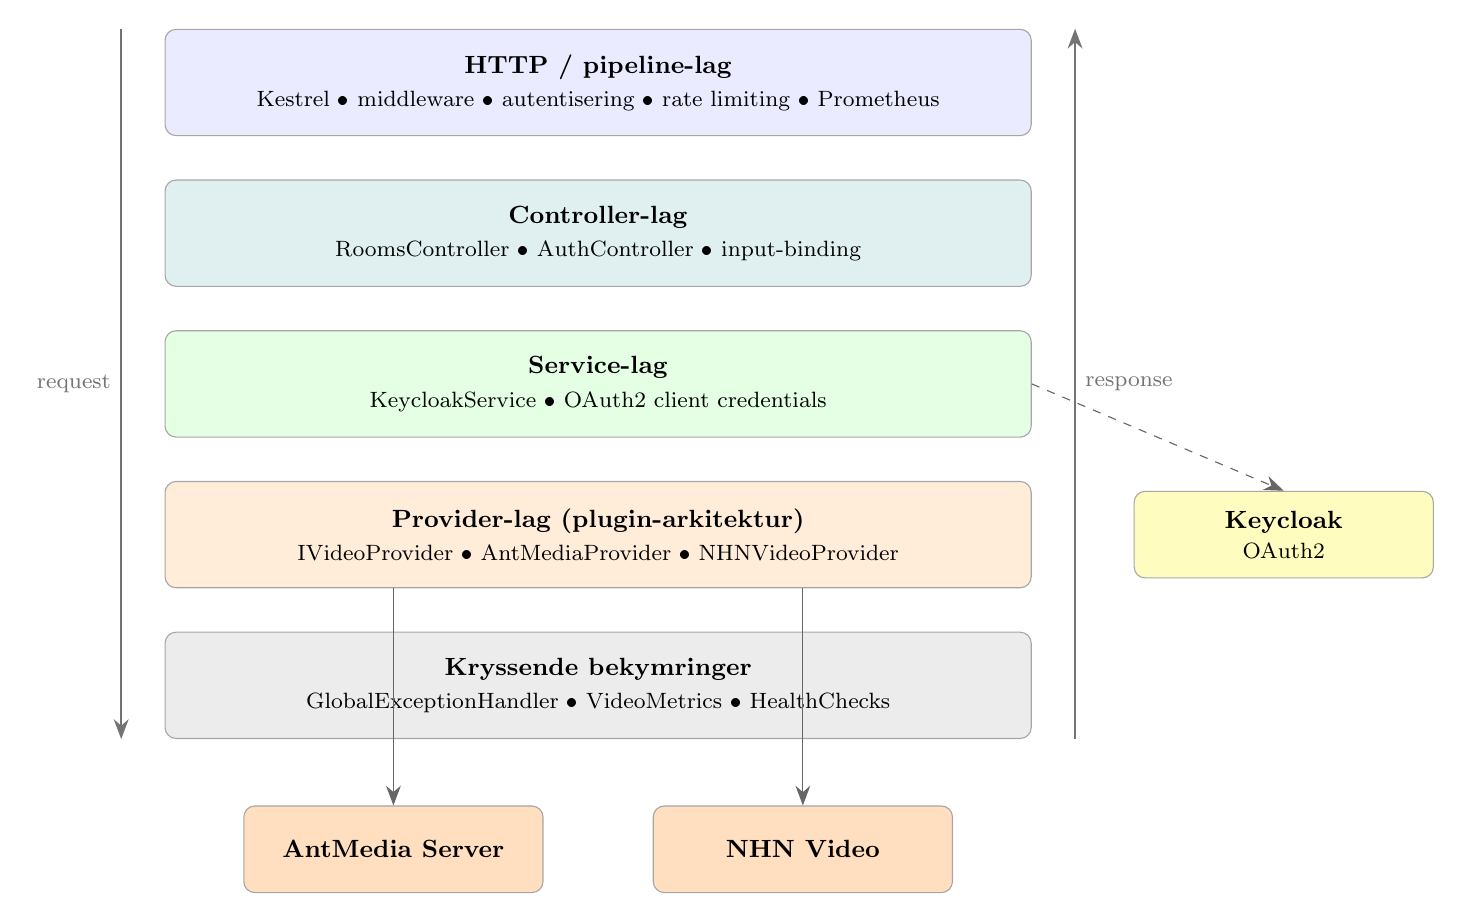
\begin{tikzpicture}[
    >={Stealth[length=2.5mm]},
    node distance=0.55cm,
    layer/.style={
        draw=black!35,
        line width=0.4pt,
        rounded corners=4pt,
        minimum width=11cm,
        minimum height=1.35cm,
        text centered,
        align=center,
        inner sep=6pt,
        font=\small
    },
    ext/.style={
        draw=black!35,
        line width=0.4pt,
        rounded corners=4pt,
        minimum width=3.8cm,
        minimum height=1.1cm,
        text centered,
        align=center,
        inner sep=4pt,
        font=\small
    },
    arrowlbl/.style={font=\footnotesize\color{black!65}}
]

% --- Layers (top to bottom) ---
\node[layer, fill=blue!8]                  (http)  {\textbf{HTTP / pipeline-lag}\\[1pt]
    {\footnotesize Kestrel \textbullet{} middleware \textbullet{} autentisering \textbullet{} rate limiting \textbullet{} Prometheus}};
\node[layer, fill=teal!12, below=of http]  (ctrl)  {\textbf{Controller-lag}\\[1pt]
    {\footnotesize RoomsController \textbullet{} AuthController \textbullet{} input-binding}};
\node[layer, fill=green!10, below=of ctrl] (svc)   {\textbf{Service-lag}\\[1pt]
    {\footnotesize KeycloakService \textbullet{} OAuth2 client credentials}};
\node[layer, fill=orange!15, below=of svc] (prov)  {\textbf{Provider-lag (plugin-arkitektur)}\\[1pt]
    {\footnotesize IVideoProvider \textbullet{} AntMediaProvider \textbullet{} NHNVideoProvider}};
\node[layer, fill=gray!15, below=of prov]  (cross) {\textbf{Kryssende bekymringer}\\[1pt]
    {\footnotesize GlobalExceptionHandler \textbullet{} VideoMetrics \textbullet{} HealthChecks}};

% --- External backends at the bottom ---
\node[ext, fill=orange!25] (ant) at ([xshift=-2.6cm, yshift=-1.4cm]cross.south) {\textbf{AntMedia Server}};
\node[ext, fill=orange!25] (nhn) at ([xshift= 2.6cm, yshift=-1.4cm]cross.south) {\textbf{NHN Video}};

% --- External service on the right (Keycloak), aligned with Service-lag ---
\node[ext, fill=yellow!25] (kc) at ([xshift=3.2cm]prov.east) {\textbf{Keycloak}\\{\footnotesize OAuth2}};


% --- Request arrow (left, downward) ---
\draw[->, thick, black!55]
    ([xshift=-0.55cm]http.north west) -- ([xshift=-0.55cm]cross.south west)
    node[midway, left, arrowlbl] {request};

% --- Response arrow (right of layer stack, upward) ---
\draw[->, thick, black!55]
    ([xshift=0.55cm]cross.south east) -- ([xshift=0.55cm]http.north east)
    node[midway, right, arrowlbl] {response};
    
% --- Provider to backends ---
\draw[->, black!60] (prov.south -| ant.north) -- (ant.north);
\draw[->, black!60] (prov.south -| nhn.north) -- (nhn.north);

% --- Service to Keycloak (dashed) ---
\draw[->, dashed, black!60] (svc.east) -- (kc.north);

\end{tikzpicture}
\caption{Overordnet lagarkitektur for HDO VideoAPI.}
\label{fig:lagarkitektur}
\end{figure}


\begin{description}
    \item[HTTP-pipeline-laget] håndterer innkommende trafikk og inneholder middleware for blant annet unntakshåndtering, HTTPS, \gls{cors}, rate limiting, JWT-autentisering, autorisasjon og Prometheus-metrikker. Disse mekanismene er lagt i pipelinen fordi de gjelder hele API-et, ikke én spesifikk romoperasjon.
    
    \item[Controller-laget] fungerer som et tynt bindeledd mellom HTTP-kontrakten og provider-laget. Controllerne binder innkommende forespørsler, velger riktig provider og returnerer HTTP-svar, men inneholder ikke backend-spesifikk logikk. Slik kan API-kontrakten holdes stabil selv om integrasjonen mot AntMedia eller NHN endres.
    
    \item[Provider-laget] er kjernen i arkitekturen. Resten av applikasjonen forholder seg til et felles \texttt{IVideoProvider}-grensesnitt, mens AntMedia- og NHN-spesifikk logikk holdes i egne provider-implementasjoner.
    
    \item[Service-laget] inneholder hjelpetjenester som brukes på tvers av provider-implementasjonene, særlig \texttt{KeycloakService} som håndterer uthenting og caching av tilgangstoken fra Keycloak.
    
    \item[Kryssende bekymringer] som feilhåndtering, metrikker og helsesjekker behandles utenfor kjerneflyten for romoperasjoner. Arkitekturen er også stateless: API-et lagrer ikke videorom eller sesjonsdata mellom forespørsler, men lar slik tilstand ligge hos de eksterne videomotorene. Dette støtter horisontal skalering og er i tråd med krav~I1.2~\cite{hdo_kravspec}.
\end{description}
\newpage
\begin{lstlisting}[language=CSharp, caption={Oppstartskonfigurasjon delegert til navngitte extension-metoder}, label={lst:program-startup}]
// HDO-VideoAPI/Program.cs

var builder = WebApplication.CreateBuilder(args);

// Konfigurasjon
builder.Configuration.AddEnvironmentVariables();            // Miljøvariabler
builder.ConfigureVideoHosting();                            // Kestrel og HTTPS

// Tjenester registreres per ansvarsdomene
builder.Services.AddVideoRateLimiting();                    // Hastighetsbegrensning
builder.Services.AddVideoApiCore();                         // Controllers, JSON, OpenAPI
builder.Services.AddVideoCors(builder.Configuration);       // CORS-policy
builder.Services.AddVideoProviders(builder.Configuration);  // Plugin-arkitektur
builder.Services.AddVideoHealthChecks(builder.Environment); // Helsesjekker 
builder.Services.AddVideoKeycloak(builder.Configuration);   // OAuth2/JWT

// Bygg og start applikasjonen
var app = builder.Build();
app.UseVideoApi();
app.Run();
\end{lstlisting}
Kodeliste~\ref{lst:program-startup} viser hvordan oppstarten er holdt kompakt ved å delegere konfigurasjon til navngitte extension-metoder. Dette gjør \texttt{Program.cs} til en oversikt over systemets hovedmoduler, i stedet for å samle all konfigurasjon i én fil.
\section{Provider-arkitektur}
\label{sec:provider-pattern}

Provider-arkitekturen er det sentrale designvalget i VideoAPI. Behovet oppstod
fordi løsningen skulle tilby ett felles API mot klientene, samtidig som kall
måtte kunne rutes til ulike videomotorer. AntMedia Server og NHN Video har ulike
API-er og domenemodeller: AntMedia eksponerer REST-endepunkter for blant annet
broadcast-ressurser, mens NHN Booking API er orientert rundt opprettelse og
administrasjon av videomøter~\cite{antmedia_rest,nhn_booking}. Samtidig stilte
kravspesifikasjonen krav om at nye videomotorer bør kunne legges til uten at hele
mellomvaren må skrives om~\cite{hdo_kravspec}.

Et alternativ var å samle all backend-logikk i én felles serviceklasse og bruke
betingelser for å skille mellom videomotorene. Dette ville vært enkelt i starten,
men ville gitt tett kobling til de konkrete backendene og gjort løsningen
vanskeligere å utvide. Et annet alternativ var å eksponere separate API-er for
hver backend, for eksempel egne endepunkter for AntMedia og NHN. Dette ville
gjort backend-forskjellene tydelige, men også flyttet kompleksiteten til
klienten, som da måtte vite hvilken videomotor som brukes og hvordan responsene
skal tolkes.

Den valgte løsningen ble derfor å definere et felles
\texttt{IVideoProvider}-grensesnitt. Hver videomotor implementeres som en egen
provider, mens controllerne kun forholder seg til grensesnittet. Designet har
likhetstrekk med adapter-mønsteret, der et felles grensesnitt brukes til å skjule
forskjeller mellom underliggende implementasjoner~\cite{refactoringguru_adapter}.
Riktig provider velges av en egen factory-komponent, slik at controllerne ikke
trenger å kjenne til de konkrete provider-klassene.

Provider-arkitekturen betyr likevel ikke at alle backendene behandles som
identiske. Enkelte operasjoner har ulik betydning i de to systemene. Start- og
stoppoperasjoner passer naturlig med AntMedia sin broadcast-modell, mens NHN
Booking API i større grad beskriver opprettelse og administrasjon av et
videomøte. Provider-laget skal derfor isolere forskjellene, ikke skjule dem helt.
Nye videomotorer kan dermed legges til ved å implementere
\texttt{IVideoProvider}, mens controllerne og klientens API-kontrakt i hovedsak
kan beholdes uendret.

\begin{lstlisting}[language=CSharp, caption={Felles provider-kontrakt}, label={lst:ivideoprovider}]
public interface IVideoProvider
{
    Task<VideoRoom> CreateRoomAsync(CreateRoomRequest request, CancellationToken ct = default);
    Task<VideoRoom> GetRoomAsync(string roomId, CancellationToken ct = default);
    Task DeleteRoomAsync(string roomId, CancellationToken ct = default);
    Task StartStreamAsync(string roomId, CancellationToken ct = default);
    Task StopStreamAsync(string roomId, CancellationToken ct = default);
    Task SetRoomTokenAsync(string roomId, string token, CancellationToken ct = default);
    Task<WebRtcLinkResponse> GenerateWebRtcTokenAsync(string roomId, string type, CancellationToken ct = default);
    Task<bool> IsAvailableAsync(CancellationToken ct = default);
}
\end{lstlisting}
Listing~\ref{lst:ivideoprovider} viser grensesnittet alle videomotorer må
implementere. Dette gjør at controller-laget kan forholde seg til én kontrakt,
mens backend-spesifikk logikk holdes i providerne.
\section{API-design}
\label{sec:api-design}

API-et er designet som et REST-basert grensesnitt der videorom er hovedressursen, i tråd med kravspesifikasjonens beskrivelse av operasjoner for oppretting, sletting, henting, start og stopp av videorom \cite{hdo_kravspec}. Alle operasjoner er samlet under \texttt{/api/rooms}, slik at klienten forholder seg til én enhetlig kontrakt uavhengig av underliggende videomotor.

% API-et er designet som et REST-basert grensesnitt der videorom er hovedressursen.
% Dette passer med kravspesifikasjonen, som beskriver operasjoner for å opprette,
% slette, hente informasjon om, starte og stoppe videorom~\cite{hdo_kravspec}.
% Operasjonene er derfor samlet under \texttt{/api/rooms}, slik at klienten får ett
% felles grensesnitt uavhengig av hvilken videomotor som brukes.

ASP.NET Core støtter både Minimal APIs og controller-baserte API-er. Minimal APIs
er anbefalt for nye prosjekter der målet er raske HTTP-endepunkter med lite
oppsett og mindre kode, mens controller-baserte API-er gir en mer strukturert
modell med egne controller-klasser, attributtbasert routing og innebygd støtte
for API-spesifikke funksjoner som modellbinding, validering og standardiserte
feilsvar~\cite{microsoft_aspnet_apis,microsoft_aspnet_webapi}. I VideoAPI ble
controller-basert API valgt fordi løsningen har flere ressursorienterte
endepunkter, felles autentisering på controller-nivå og behov for tydelig
separasjon mellom HTTP-kontrakt og provider-logikk. Minimal APIs kunne vært brukt
for en mindre prototype, men controller-modellen ga en tydeligere struktur for
operasjoner som oppretting, sletting, start, stopp, tokenhåndtering og
WebRTC-lenker for videorom.

VideoAPI eksponerer utelukkende et server-side REST API over HTTP uten
klientbibliotek. Primære konsumenter er backend-tjenester og operatørapplikasjoner;
enhver HTTP-klient kan integrere mot det. AntMedia og NHN er de to videomotorene
som er implementert i proof-of-concept-et, men provider-arkitekturen er designet
for at nye motorer kan legges til uten endringer i API-kontrakten
(jf.\ avsnitt~\ref{sec:provider-validering}).

Et sentralt designvalg var hvordan API-et skulle bevare informasjon om hvilken backend et rom tilhører. Løsningen ble å returnere rom-ID-er på formatet \texttt{\{provider\}:\{backendId\}}, for eksempel \texttt{antmedia:abc123} eller \texttt{nhn:24484}. Provider-prefikset fungerer som rutinginformasjon i senere forespørsler, slik at klienten kun trenger å lagre én ID. Kodeliste~\ref{lst:create-room} viser at controlleren holdes tynn: den binder forespørselen, velger provider, delegerer romopprettelsen og prefikser rom-ID-en før svaret returneres.
\begin{lstlisting}[language=CSharp, caption={Opprettelse av rom — controlleren delegerer til provider-laget.}, label={lst:create-room}]
// HDO-VideoAPI/Controllers/RoomsController.cs

[HttpPost]
public async Task<IActionResult> CreateRoom([FromBody] CreateRoomRequest request)
{
    // ... (genere navn om ikke oppgitt)

    // Velg provider basert på forespørsel, standardverdi er antmedia
    var providerKey = (request.Provider ?? "antmedia").ToLowerInvariant();
    var provider = factory.GetProvider(providerKey);

    // Deleger romoppretting til provider-laget
    var room = await provider.CreateRoomAsync(request, HttpContext.RequestAborted);

    // Prefiks ID med provider-nøkkel
    room.Id = $"{providerKey}:{room.Id}";

    // ... (logging)

    // Returnere 201 Created med Location-header
    return CreatedAtAction(nameof(GetRoom), new { roomId = room.Id }, room);
}
\end{lstlisting}

Ved senere kall — henting, sletting, start og stopp — må controlleren gjenkjenne hvilken provider rom-ID-en tilhører. Kodeliste~\ref{lst:parse-room-id} viser hvordan provider-prefikset parses ut av ID-en, slik at provider-valget ikke trenger å sendes som et eget felt eller query-parameter.

\begin{lstlisting}[language=CSharp, caption={Parsing av provider-prefiks fra rom-ID}, label={lst:parse-room-id}]
// HDO-VideoAPI/Controllers/RoomsController.cs

private (IVideoProvider Provider, string ProviderKey, string RawId) ParseRoomId(string roomId)
{
    // Finn skilletegnet mellom provider og backend-ID
    var colon = roomId.IndexOf(':');

    // ... (valider at kolon finnes)

    var providerKey = roomId[..colon];  // f.eks. "antmedia"
    var rawId = roomId[(colon + 1)..];  // f.eks. "abc123"

    // ... (valider at rawId ikke er tom)

    // Slå opp provider og returner alle tre delene
    return (factory.GetProvider(providerKey), providerKey, rawId);
}
\end{lstlisting}

Start og stopp av videostrøm er modellert som handlinger på romressursen, for
eksempel \texttt{POST /api/rooms/\{roomId\}/start} og
\texttt{POST /api/rooms/\{roomId\}/stop}. Dette ble valgt fordi operasjonene
alltid gjelder et bestemt rom. Samtidig gir ikke alle operasjoner mening for alle
backends. AntMedia har en broadcast-modell der start og stopp passer naturlig,
mens NHN Booking API i større grad beskriver et videomøte som er klart etter
opprettelse. Slike forskjeller håndteres i provider-laget.

API-et bruker JSON for forespørsler og svar, og responsmodellene er normalisert
så langt det er hensiktsmessig. Klienten får samme overordnede struktur
uavhengig av backend, men backend-spesifikke forskjeller skjules ikke dersom de
påvirker hvordan operasjonen må brukes. Dette gjelder særlig WebRTC-lenker:
AntMedia returnerer en kortlivet tokenbasert tilgang til streamen, mens NHN
returnerer en møte-URL med tilgangsinformasjon.

Feilresponsene er også standardisert. Dersom en provider ikke støtter en
operasjon, eller en ekstern backend returnerer feil, oversettes dette til et
strukturert HTTP-svar gjennom den globale feilhåndteringen. Dette gjør at
controllerne kan være like for alle providere, mens klienten fortsatt får
forutsigbare HTTP-statuskoder og feilmeldinger.
\section{Datamodeller}
\label{sec:datamodeller}

Datamodellene i VideoAPI er utformet for å gi klienten et stabilt og
backend-uavhengig grensesnitt. Siden AntMedia og NHN representerer videorom på
ulike måter, eksponeres ikke råresponsene fra backendene direkte. I stedet mapper
providerne backend-spesifikke svar til felles modeller som kan brukes på tvers av
videomotorene.

Den viktigste responsmodellen er \texttt{VideoRoom}. Modellen representerer et
videorom slik VideoAPI eksponerer det til klienten, med blant annet rom-ID,
provider, status og relevante tilkoblingsfelter. For AntMedia bygges modellen fra
broadcast-data, mens den for NHN bygges fra booking-data. Dette gjør at klienten
kan forholde seg til samme responsstruktur, selv om backendene har ulike
domenemodeller.

Ved opprettelse av rom brukes \texttt{CreateRoomRequest}. Denne modellen
inneholder valgt provider og valgfritt romnavn. Dersom klienten ikke angir navn,
genererer mellomvaren et unikt navn. Dette er i tråd med kravspesifikasjonen,
som beskriver at mellomvaren skal sette navn eller ID dersom dette ikke sendes
med av klienten~\cite{hdo_kravspec}.

For tilgang til videorom brukes \texttt{WebRtcLinkResponse}. Denne modellen
normaliserer to ulike tilgangsformer. AntMedia returnerer en kortlivet
tokenbasert tilgang til en stream, mens NHN returnerer en møte-URL med nødvendig
tilgangsinformasjon. Modellen gir derfor klienten ett felles svarformat, men
uten å skjule at verdien må brukes forskjellig avhengig av backend.

Datamodellene er dermed et kompromiss mellom standardisering og presisjon. De
skjuler unødvendige forskjeller fra klienten, men lar backend-spesifikke
forskjeller komme frem der de påvirker hvordan operasjonen faktisk brukes.
\section{Sikkerhetsarkitektur}
\label{sec:design-sikkerhet}
Dette delkapittelet beskriver sikkerhetsdesignet i VideoAPI. Først gjennomgås autentisering og tilgangskontroll, inkludert valg av Keycloak og OAuth2-flyt. Deretter beskrives claim-struktur og tokenvalidering, før det avsluttes med en gjennomgang av utvalgte angrepsscenarier og tilhørende kontroller. En STRIDE-basert trusselmodell finnes i delkapittel~\ref{sec:trusselmodell}.

\subsection{Autentisering og tilgangskontroll}

Autentisering i VideoAPI er basert på OAuth2-standarden, noe som var et eksplisitt krav fra oppdragsgiver. Valget av OAuth2 gir en industristandard tilnærming til tilgangskontroll som er vidt støttet og godt dokumentert, og som muliggjør fremtidig integrasjon med andre systemer uten behov for endringer i API-ets grensesnitt.

\subsection{Valg av Keycloak som identitetsleverandør}

Som OAuth2-leverandør ble Keycloak valgt. Bakgrunnen for dette valget er at HDO allerede benytter Keycloak som identity provider i sin eksisterende infrastruktur. Ved å ta i bruk det samme systemet unngikk gruppen å innføre ny teknologi i driftsmiljøet, og oppdragsgiver kan selv ta over og tilpasse konfigurasjonen i etterkant uten å måtte sette seg inn i et ukjent verktøy.

Autentiseringsmekanismen er implementert ved bruk av OAuth 2.0-flyten \textit{Client Credentials Grant}, også omtalt som \gls{m2m}-autentisering. Denne flyten er passende for et API uten sluttbrukerpålogging, der klientsystemer autentiserer seg med en klient-ID og klienthemmelighet for å hente et JWT-token. Tokenet brukes deretter som \texttt{Bearer}-token i alle påfølgende API-kall.

\subsection{Minimal claim-struktur}

Et bevisst designvalg i autentiseringsarkitekturen er å holde claim-strukturen enkel. Det er kun én claim som kreves for tilgang: \texttt{api\_access = true}. Det er ikke benyttet OAuth2-scopes.

Denne forenklingen er begrunnet i prosjektets kontekst: autentiseringsoppsettet er ment som et midlertidig rammeverk som oppdragsgiver selv skal overta og konfigurere videre med sin egen Keycloak-instans. Å designe et komplekst scope-hierarki som senere ville blitt erstattet ville ført til unødvendig arbeid uten varig verdi. Den enkelte \texttt{api\_access}-claimen fungerer derfor som en enkel binær tilgangskontroll, hvor en klient enten gis tilgang eller avvises.

Keycloak-klienter som skal ha tilgang til API-et må konfigureres med en protokollmapper som legger til denne claimet i tokens som utstedes. Selve policy-sjekken skjer globalt i API-ets autorisasjonsmiddleware, slik at alle beskyttede endepunkter automatisk krever gyldig token med riktig claim uten at dette må defineres eksplisitt per endepunkt.

\subsection{Validering og sikkerhetsnivå}

JWT-tokens valideres mot Keycloaks JWKS-endepunkt, som betyr at signaturen verifiseres med Keycloaks offentlige nøkkel ved hvert kall. Audience- og issuer-validering er i det nåværende oppsettet deaktivert, da disse parameterne vil variere avhengig av hvilken Keycloak-instans oppdragsgiver velger å benytte. Signaturvalidering sikrer at tokens ikke kan forfalskes, og at kun tokens utstedt av den konfigurerte Keycloak-realmen godtas.

\subsection{Utvalgte angrep og kontroller}

Token-endepunktet \texttt{POST /auth/token} er beskyttet med en skjerpet
rate-limit på 10 forespørsler per minutt per IP-adresse, sammenlignet med
den generelle grensen på 60 forespørsler per minutt. Dette er et tiltak
mot credential-stuffing og ressursuttømming mot autentiseringslaget.

% Autorisasjonsmodellen er flat: enhver klient med gyldig JWT og
% \texttt{api\_access}-claim har samme rettigheter. Rom-ID-er er derfor ikke
% personlige hemmeligheter i seg selv. Dersom en klient kjenner en annen
% klients rom-ID, kan den i prinsippet kalle rom-endepunktene, med mindre
% dette hindres utenfor VideoAPI. Rom-spesifikk isolasjon mellom
% integrasjonsparter er utenfor proof-of-conceptets omfang, men dokumenteres
% her som en bevisst avgrensning.

Autorisasjonsmodellen er flat: enhver klient med gyldig JWT og \texttt{api\_access}-claim tildeles samme rettigheter. Rom-ID-er betraktes derfor ikke som personlige hemmeligheter i seg selv. Dersom en klient kjenner en annen klients rom-ID, kan den i prinsippet benytte rom-endepunktene, med mindre dette begrenses av mekanismer utenfor VideoAPI. Romspesifikk isolasjon mellom integrasjonsparter ligger utenfor POC-ets omfang og er dokumentert som en bevisst avgrensning.

En STRIDE-basert oppsummering av trusler og tiltak finnes i
delkapittel~\ref{sec:trusselmodell}.
\section{Sekvensdiagrammer}
\label{sec:sekvensdiagram}

Figur~\ref{fig:sekvens-opprette-rom} viser opprettelse av videorom ut fra klientens
perspektiv. Flyten forutsetter at klienten allerede har hentet et gyldig
Bearer-token fra \texttt{/auth/token}, som beskrevet i
avsnitt~\ref{sec:design-sikkerhet}; alle romkall i diagrammet antar gyldig JWT med
påkrevd claim.

\usetikzlibrary{positioning,arrows.meta,calc}
\begin{figure}[htbp]
\centering
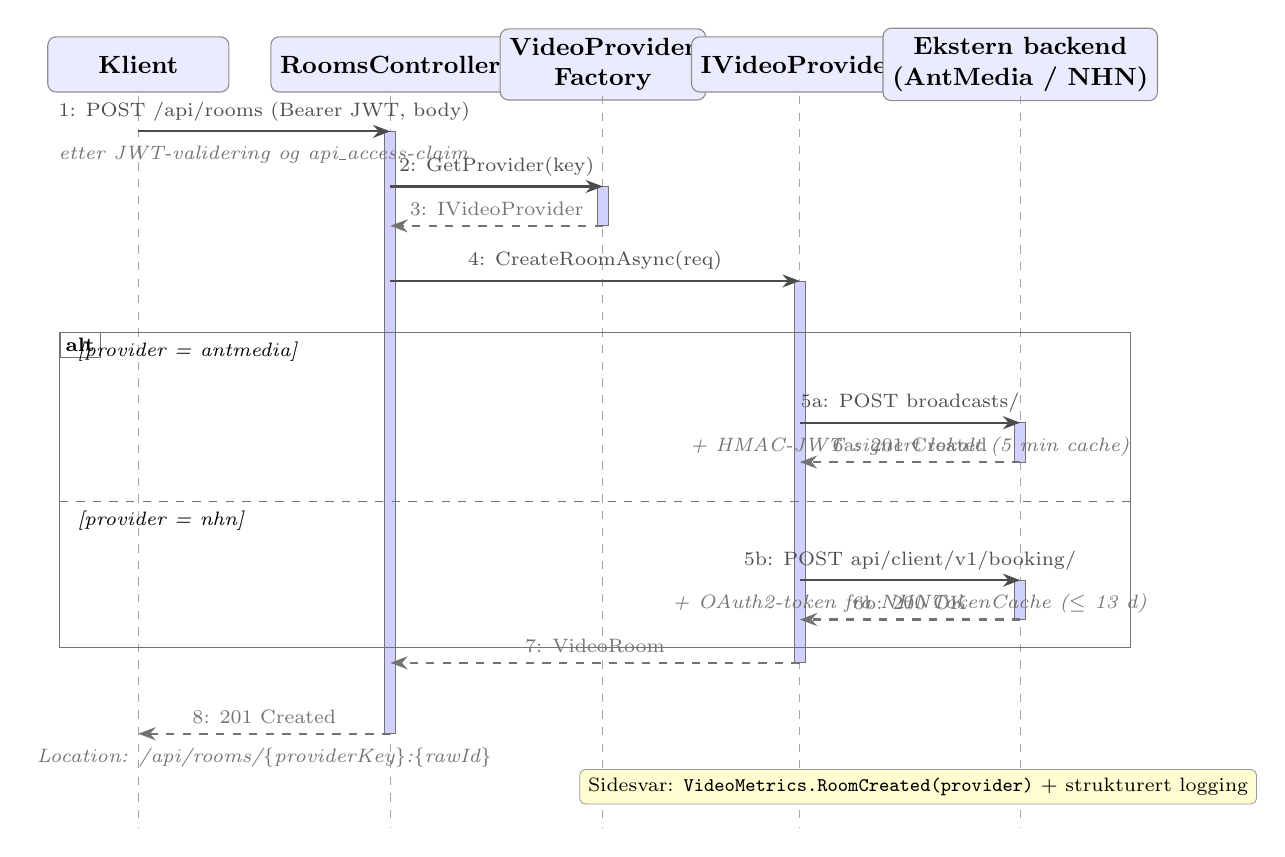
\begin{tikzpicture}[
    >={Stealth[length=2.2mm]},
    actor/.style={
        draw=black!45,
        rounded corners=3pt,
        line width=0.4pt,
        minimum width=2.3cm,
        minimum height=0.7cm,
        fill=blue!8,
        align=center,
        font=\small\bfseries
    },
    msg/.style={->, thick, black!70, font=\footnotesize},
    ret/.style={->, thick, dashed, black!55, font=\footnotesize},
    activ/.style={draw=black!55, fill=blue!18, line width=0.3pt},
    altframe/.style={draw=black!55, line width=0.4pt},
    altlbl/.style={fill=white, draw=black!55, line width=0.3pt, font=\scriptsize\bfseries, inner sep=2pt},
    altsep/.style={dashed, black!55, line width=0.4pt},
    note/.style={draw=black!40, fill=yellow!18, line width=0.3pt, font=\scriptsize, align=left, inner sep=3pt, rounded corners=2pt}
]

% --- Lifeline x-positions ---
\def\xKli{0}
\def\xCtrl{3.2}
\def\xFact{5.9}
\def\xProv{8.4}
\def\xBack{11.2}

% --- Actor headers ---
\node[actor] (kli)  at (\xKli,  0) {Klient};
\node[actor] (ctrl) at (\xCtrl, 0) {RoomsController};
\node[actor] (fact) at (\xFact, 0) {VideoProvider\\Factory};
\node[actor] (prov) at (\xProv, 0) {IVideoProvider};
\node[actor] (back) at (\xBack, 0) {Ekstern backend\\(AntMedia / NHN)};

% --- Lifelines ---
\def\bottomy{-9.7}
\foreach \x in {\xKli,\xCtrl,\xFact,\xProv,\xBack}
    \draw[dashed, black!35] (\x, -0.4) -- (\x, \bottomy);

% --- Activation bars ---
\fill[activ] (\xCtrl-0.07, -0.85) rectangle (\xCtrl+0.07, -8.5);
\fill[activ] (\xFact-0.07, -1.55) rectangle (\xFact+0.07, -2.05);
\fill[activ] (\xProv-0.07, -2.75) rectangle (\xProv+0.07, -7.6);
\fill[activ] (\xBack-0.07, -4.55) rectangle (\xBack+0.07, -5.05);
\fill[activ] (\xBack-0.07, -6.55) rectangle (\xBack+0.07, -7.05);

% --- Messages ---
% 1. Klient -> Controller
\draw[msg] (\xKli, -0.85) -- (\xCtrl, -0.85)
    node[midway, above, font=\scriptsize] {1: POST /api/rooms (Bearer JWT, body)};
\node[font=\scriptsize, black!55] at ($(\xKli, -0.85)!0.5!(\xCtrl, -0.85) + (0,-0.30)$)
    {\textit{etter JWT-validering og api\_access-claim}};

% 2. Controller -> Factory
\draw[msg] (\xCtrl, -1.55) -- (\xFact, -1.55)
    node[midway, above, font=\scriptsize] {2: GetProvider(key)};

% 3. Factory -> Controller (return)
\draw[ret] (\xFact, -2.05) -- (\xCtrl, -2.05)
    node[midway, above, font=\scriptsize] {3: IVideoProvider};

% 4. Controller -> Provider
\draw[msg] (\xCtrl, -2.75) -- (\xProv, -2.75)
    node[midway, above, font=\scriptsize] {4: CreateRoomAsync(req)};

% --- alt fragment ---
\draw[altframe] (\xKli-1.0, -3.4) rectangle (\xBack+1.4, -7.4);
\node[altlbl, anchor=north west] at (\xKli-1.0, -3.4) {alt};

% [antmedia] branch
\node[font=\scriptsize\itshape, anchor=west] at (\xKli-0.9, -3.65) {[provider = antmedia]};

% 5a. Provider -> Backend (AntMedia)
\draw[msg] (\xProv, -4.55) -- (\xBack, -4.55)
    node[midway, above, font=\scriptsize] {5a: POST broadcasts/};
\node[font=\scriptsize, black!55] at ($(\xProv, -4.55)!0.5!(\xBack, -4.55) + (0,-0.30)$)
    {\textit{+ HMAC-JWT signert lokalt (5 min cache)}};

% 6a. Backend -> Provider (return)
\draw[ret] (\xBack, -5.05) -- (\xProv, -5.05)
    node[midway, above, font=\scriptsize] {6a: 201 Created};

% --- separator ---
\draw[altsep] (\xKli-1.0, -5.55) -- (\xBack+1.4, -5.55);
\node[font=\scriptsize\itshape, anchor=west] at (\xKli-0.9, -5.80) {[provider = nhn]};

% 5b. Provider -> Backend (NHN)
\draw[msg] (\xProv, -6.55) -- (\xBack, -6.55)
    node[midway, above, font=\scriptsize] {5b: POST api/client/v1/booking/};
\node[font=\scriptsize, black!55] at ($(\xProv, -6.55)!0.5!(\xBack, -6.55) + (0,-0.30)$)
    {\textit{+ OAuth2-token fra NHNTokenCache ($\le$ 13 d)}};

% 6b. Backend -> Provider (return)
\draw[ret] (\xBack, -7.05) -- (\xProv, -7.05)
    node[midway, above, font=\scriptsize] {6b: 200 OK};

% --- end alt ---

% 7. Provider -> Controller (return)
\draw[ret] (\xProv, -7.6) -- (\xCtrl, -7.6)
    node[midway, above, font=\scriptsize] {7: VideoRoom};

% 8. Controller -> Klient (return)
\draw[ret] (\xCtrl, -8.5) -- (\xKli, -8.5)
    node[midway, above, font=\scriptsize] {8: 201 Created};
\node[font=\scriptsize, black!55] at ($(\xKli, -8.5)!0.5!(\xCtrl, -8.5) + (0,-0.30)$)
    {\textit{Location: /api/rooms/\{providerKey\}:\{rawId\}}};

% --- Side-effect note ---
\node[note, anchor=north west] at (\xFact-0.3, -8.95)
    {Sidesvar: \texttt{VideoMetrics.RoomCreated(provider)} + strukturert logging};

\end{tikzpicture}
\caption{Sekvensdiagram for opprettelse av videorom. Controlleren er provider-agnostisk: \texttt{VideoProviderFactory} løser opp riktig \texttt{IVideoProvider} via keyed dependency injection, og en \texttt{DelegatingHandler} på provider-laget håndterer den backend-spesifikke autentiseringen. \texttt{alt}-fragmentet viser hvor abstraksjonen brytes: AntMedia signerer en kortlevd JWT lokalt (HMAC-SHA256, 5 minutters cache), mens NHN bruker et OAuth2-token fra \texttt{NHNTokenCache} med levetid på inntil 13 dager.}
\label{fig:sekvens-opprette-rom}
\end{figure}


\section{Trusselmodell og avveininger}
\label{sec:trusselmodell}

Tabell~\ref{tab:stride-videoapi} gir en oversikt over representative trusler mot
VideoAPI, innførte tiltak og bevisste begrensninger i proof-of-concept-et,
organisert etter STRIDE-kategoriene~\cite{stride_ms}.

\begin{table}[htbp]
\centering
\caption{STRIDE-orientert oversikt over trusler, tiltak og merknader for VideoAPI.}
\label{tab:stride-videoapi}
\begin{tabular}{p{2.8cm} p{5.0cm} p{7.2cm}}
\toprule
\textbf{STRIDE} & \textbf{Trussel} & \textbf{Tiltak og merknader} \\
\midrule

Spoofing &
Falske tokens eller klienter som utgir seg for legitime aktører. &
JWT-signatur verifiseres mot Keycloaks JWKS-endepunkt.
Issuer- og audience-validering er deaktivert i POC-et for å gjøre det enklere
å bytte Keycloak-instans; bør aktiveres i produksjon. \\

\addlinespace[6pt]

Tampering &
Trafikk eller nyttelaster endres underveis. &
TLS i drift; JWT-signaturen dekker autorisasjonsdata. \\

\addlinespace[6pt]

Repudiation &
En klient benekter å ha utført en handling. &
Strukturert logging og \texttt{traceId} i feilsvar gir delvis sporbarhet.
Fullstendig revisjonslogg er ikke implementert. \\

\addlinespace[6pt]

Information disclosure &
Hemmeligheter eller pasientdata lekker til logger eller klient. &
JWT, API-nøkler og pasientinformasjon logges ikke
(jf.\ avsnitt~\ref{sec:errors}). Feilsvar med statuskode \texttt{5xx}
inneholder kun generisk tekst. \\

\addlinespace[6pt]

Denial of service &
Ressursuttømming mot token- eller rom-endepunkter. &
Rate limiting globalt og skjerpet mot \texttt{/auth/token}.
Stateless design gjør horisontal skalering mulig. \\

\addlinespace[6pt]

Elevation of privilege &
En klient får tilgang til andre klienters rom. &
Flat tilgangsmodell: alle med gyldig \texttt{api\_access}-token
har identiske rettigheter. En klient som kjenner en annen klients
rom-ID kan i prinsippet operere på den — skille mellom leietakere
er utenfor POC-omfanget. \\

\bottomrule
\end{tabular}
\end{table}

Signaturvalidering gir beskyttelse mot token-forfalskning, men deaktivert
issuer/audience-sjekk og flat autorisasjon er teknisk gjeld som bør adresseres
før produksjonssetting.
